\color{blue}

\section{Evaluation}

\subsection{Hypotheses Formulation}

We formulate the following hypotheses to evaluate the effectiveness of our approach:

\textbf{H1:} The introduction of dynamic topological features can effectively improve the recognizability of CCGs.

\textbf{H2:} \dots

\subsection{Participants}

We recruited X participants, [add demographic analysis here].

\subsection{Datasets}

We used the following datasets for our evaluation:

\begin{itemize}
    \item Under 75 mortality from cardiovascular disease
    \item Emergency admissions for alcohol-related liver disease
\end{itemize}

135 CGGs are projected on the screen with a choropleth, we then generated another view with our visual design. The color in both visualizations are mapped to population. See \autoref{fig:task}.

{
    \begin{figure}[tb!]
        \centering
        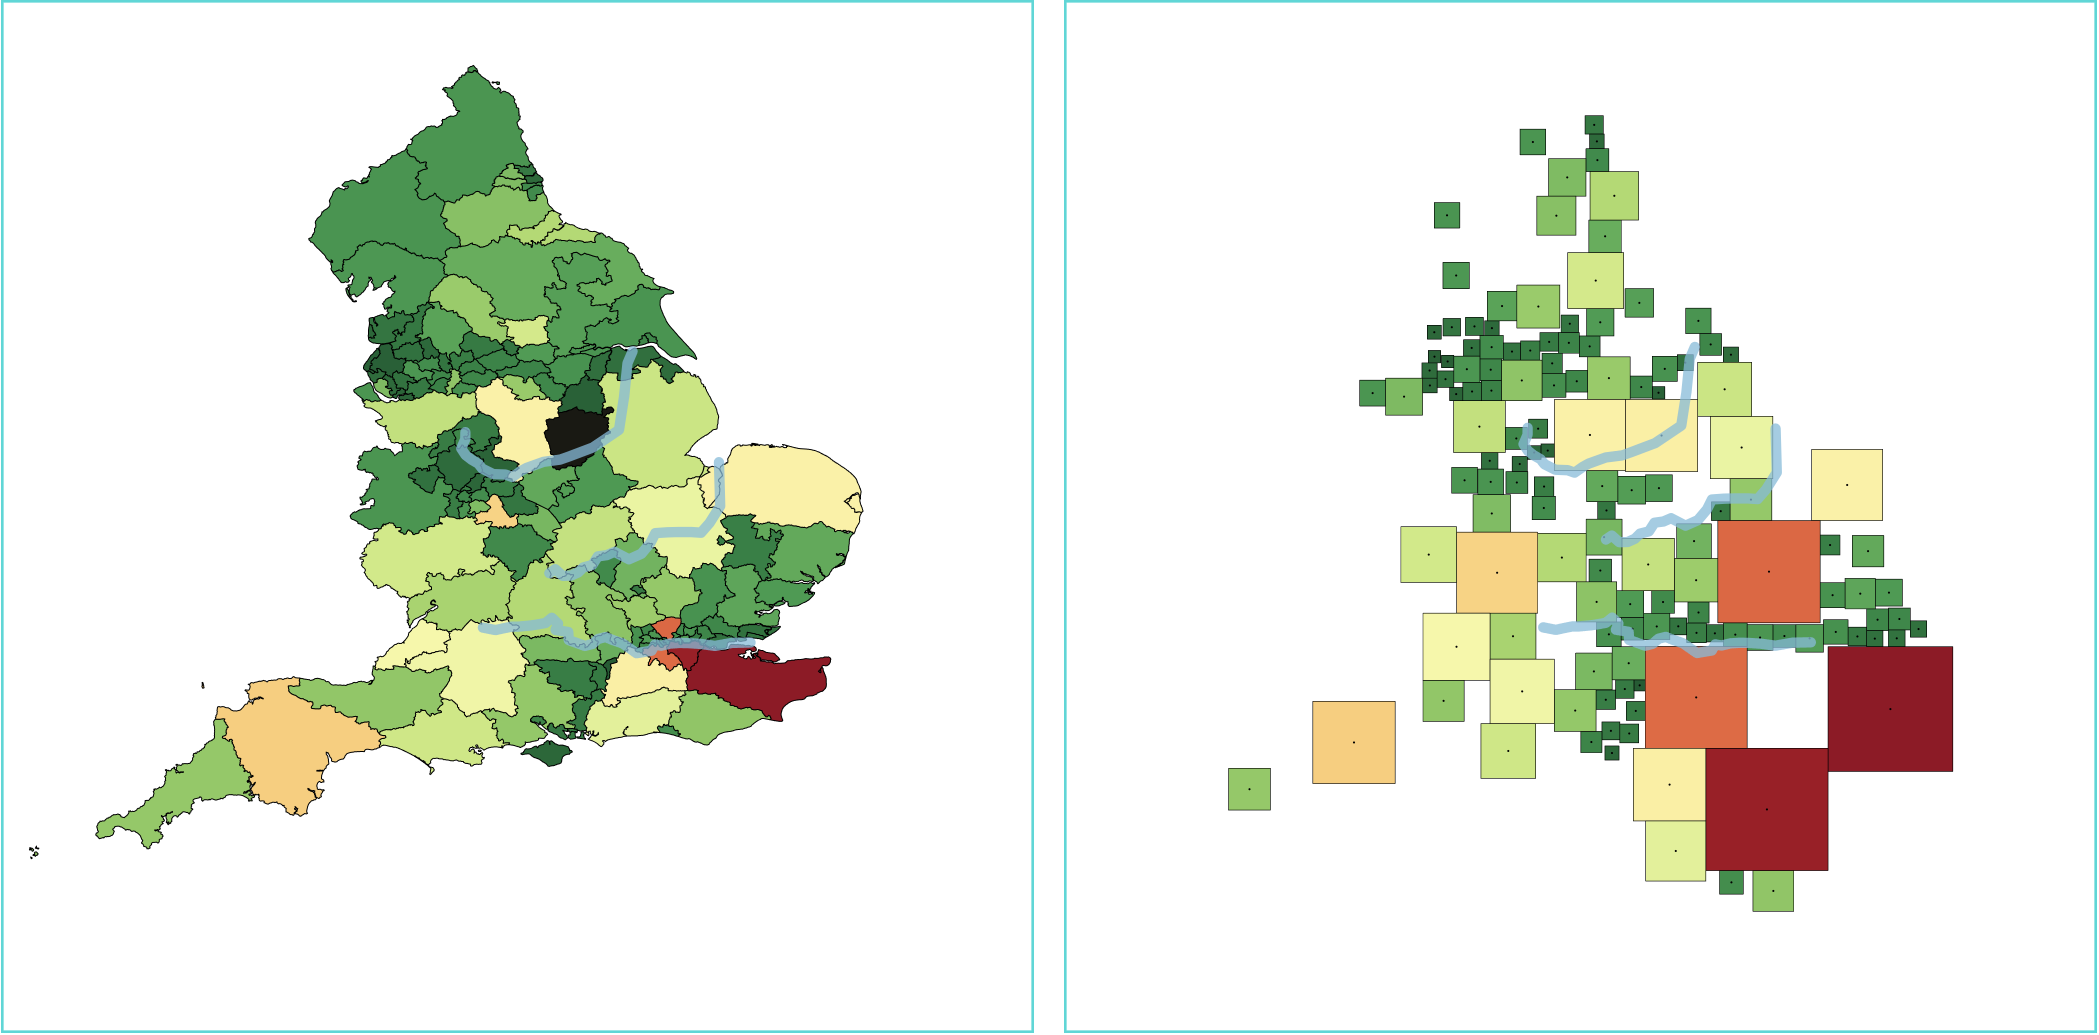
\includegraphics[width=\columnwidth,keepaspectratio]{figure/evaluation/task.png}
        \caption{A typical task for participants. The left shows the choropleth map, and the right shows the cartogram. Both visualizations show the three longest rivers in England, and the color is mapped to CCG population. The target CGG will be blinking on the choropleth (shown in black), participants are asked to identify this CCG on the cartogram.}
        \label{fig:task}
    \end{figure}
}

\subsection{User Experiment}

We conducted a user experiment to evaluate the effectiveness of our approach. The experiment was designed to be conducted remotely, and participants were asked to complete the tasks on their own computers. The experiment includes four parts:

\textbf{P1:} The participants were asked read instructions and trainings provided in both text and videos. The instructions were designed to help participants understand the concepts used in the tasks. Videos are available at \url{https://www.youtu.be/playlist?list=PLL7sHvxLtD75fMtrUQrAdddjt3wfFkcWz}.

\textbf{P2:} The participants were given three practice tasks to familiarize themselves with the experiment. A demonstration of the task is also included in the instructional video.

\textbf{P3:} The participants were asked to complete 16 location tasks. The response and reaction time are recorded. These 16 CCGs were carefully selected to avoid extreme cases (thus biases the result), in terms of size, color, and location.

\textbf{P4:} The participants were asked to complete a questionnaire that consists of Likert Scale questions and open-ended questions.

The user experiment is available at \url{https://osf.io/q39w7}.

\color{black}